\documentclass{article}
\usepackage[utf8]{inputenc}
\usepackage[english,bulgarian,ukrainian,russian]{babel}
\usepackage{a4wide}

\title{17. Наивный байесовский алгоритм, метод k ближайших соседей. Калибровка вероятностей}
\author{Kazakbaev Rustem}
\date{December 2020}

\usepackage{natbib}
\usepackage{graphicx}

\begin{document}

\maketitle


\section{Наивный Байесовский классификатор}
\textbf{Наивный байесовский классификатор} – это алгоритм классификации, основанный на теореме Байеса с допущением о независимости признаков.

Пример: фрукт может считаться яблоком, если:
\begin{itemize}
    \item Он красный
    \item Круглый
    \item Его диаметр составляет порядка 8 см
\end{itemize}
Предполагаем, что признаки вносят независимый вклад в вероятность ответа.

Теорема Байеса:
\begin{equation}
    P(c|x) = \frac{P(x|c) \cdot P(c)}{P(x)}
\end{equation}

\subsection{Пример работы}
На основе данных о погоде определить состоится или не состоится матч.

\begin{tabular}{|l|l|}
\hline Weather & Play \\
\hline Sunny & No \\
\hline Overcast & Yes \\
\hline Rainy & Yes \\
\hline Sunny & Yes \\
\hline Sunny & Yes \\
\hline Overcast & Yes \\
\hline Rainy & No \\
\hline Rainy & No \\
\hline Sunny & Yes \\
\hline Rainy & Yes \\
\hline Sunny & No \\
\hline Overcast & Yes \\
\hline Overcast & Yes \\
\hline Rainy & No \\
\hline
\end{tabular}

Как будем применять теорему Байеса? Вначале преобразуем данные

\begin{tabular}{|l|l|l|l|} 
\hline Weather & No & Yes & P \\
\hline Overcast & 0 & 4 & $\frac{4}{14}$ \\
\hline Rainy & 3 & 2 & $\frac{5}{14}$ \\
\hline Sunny & 2 & 3 & $\frac{5}{14}$\\
\hline Grand Total & 5 & 9 \\
\hline Total & $\frac{5}{14}$ & $\frac{9}{14}$ \\
\hline
\end{tabular}

Формализуем задачу:

\begin{equation}
    P(Yes|Sunny) = \frac{P(Sunny|Yes) \cdot P(Yes)}{P(Sunny)}
\end{equation}

В таком случае: $P(Yes|Sunny) = \frac{3/9*9/14}{5/14} = 0.6$.

Итак, с вероятностью 60\% будет матч при солнечной погоде. 

Для каждого набора значения признаков вычисляем вероятность ответа и берем тот ответ, для которого вероятность наибольшая

\subsection{Преимущества и недостатки}
Аналогичным образом с помощью наивного байесовского алгоритма можно прогнозировать несколько различных классов на основе множества признаков.
Преимущества
\begin{itemize}
    \item Классификация быстрая и простая
    \item В случае, если выполняется предположение о независимости, классификатор показывает очень высокое качество
\end{itemize}

Недостатки
\begin{itemize}
    \item Eсли в тестовых данных присутствует категория, не встречавшаяся в данных для обучения, модель присвоит ей нулевую вероятность
\end{itemize}

\section{Метод ближайших соседей}
\textbf{Идея:} схожие объекты находятся близко друг к другу в пространстве признаков.

Как классифицировать?

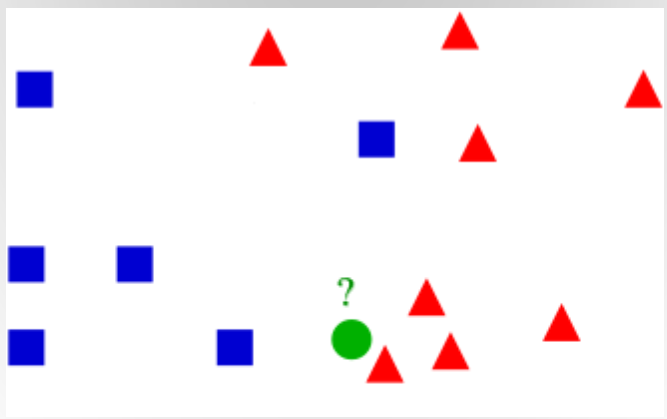
\includegraphics[scale=0.3]{nghb.png}

Формализуем, что значит ближе к треугольнику

Чтобы классифицировать новый объект, нужно:
\begin{itemize}
    \item Вычислить расстояние до каждого из объектов обучающей выборки.
    \item Выбрать k объектов обучающей выборки, расстояние до которых минимально.
    \item Класс классифицируемого объекта — это класс, наиболее часто встречающийся среди k ближайших соседей.
\end{itemize}

Число ближайших соседей k – гиперпараметр метода. Например, для k = 4 получим:

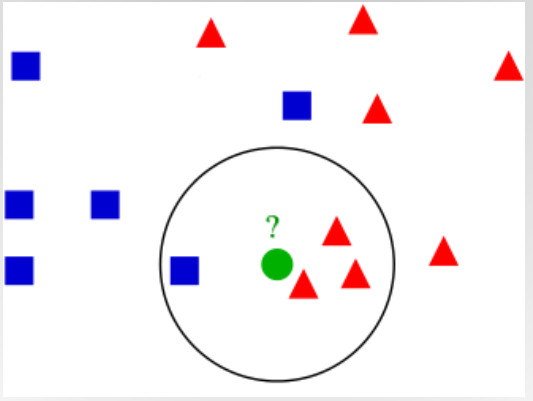
\includegraphics[scale=0.3]{sol.png}

То есть объект будет отнесён к классу треугольников.

Пусть $k$ - количество соседей. Для каждого объекта $u$
возьмём $k$ ближайших к нему объектов из тренировочной
выборки:
$$
x_{(1 ; u)}, x_{(2 ; u)}, \ldots, x_{(k ; u)}
$$
Тогда класс объекта $u$ определяется следующим образом:
$$
\boldsymbol{a}(\boldsymbol{u})=\underset{\boldsymbol{y} \in \boldsymbol{Y}}{\operatorname{argmax}} \sum_{i=1}^{\boldsymbol{k}}\left[\boldsymbol{y}\left(\boldsymbol{x}_{(i ; \boldsymbol{u})}\right)=\boldsymbol{y}\right]
$$

Ближайшие объекты – это объекты, расстояние от которых до данного объекта наименьшее по некоторой метрике $\rho$.

\begin{itemize}
    \item В качестве метрики $\rho$ как правило используют евклидово расстояние, но можно использовать и другие метрики.
    \item Перед использованием метода необходимо масштабировать данные, иначе признаки с большими числовыми значениями будут доминировать при вычислении расстояний.
\end{itemize}

Иногда еще рассматривают соседей с весами. Присваивают вес в зависимости от расстояния. Чем дальше объект тем меньше у него вес.

Как правило, метод не очень хорошо работает. Его лучше использовать в качестве бейзлайна.

\section{Калибровка вероятностей}
\textbf{Калибровка вероятностей} - приведение ответов алгоритма к значениям, близким к вероятностям объектов принадлежать конкретному классу. Мера уверенности алгоритма и вероятность это разные вещи.

Зачем?
\begin{itemize}
    \item Вероятности гораздо проще интерпретировать
    \item Вероятности могут дать дополнительную информацию о результатах работы алгоритма
\end{itemize}

Идея: обучаем логистическую регрессию на ответах классификатора a(x).

Формализуем задачу:
\begin{itemize}
    \item Пусть есть два класса: $Y=\{+1, -1\}$
\end{itemize}

Задача: для классификатора a(x), предсказывающего значения из отрезка [0, 1], либо предсказывающего класс (+1 или -1), сделать калибровку, чтобы предсказания быди вероятностями $p(y=+1|x).$

$\pi(x ; \alpha ; \beta)=\sigma(\alpha \cdot a(x)+\beta)=\frac{1}{1+e^{-(\alpha \cdot a(x)+\beta)}}$

a(x) это предсказание нашего классификатора. Предсказание станет новым признаком, тогда мы берем некоторые веса и применяем сигмоиду.

Очевидно, что алгоритм лучше работать не будет. Сами меры уверенности будут ближе к вероятности. Это важно исключительно для интерпретации.

Находим $\alpha$ и $\beta$, минимизируя логистическую функцию потерь (то есть обучаем логистическую регрессию):

$-\sum_{y_{i}=-1} \log (1-\pi(x ; \alpha ; \beta))-\sum_{y_{i}=+1} \log (\pi(x ; \alpha ; \beta)) \rightarrow \min _{\alpha, \beta}$


\end{document}
